\chapter{Trabalhos Relacionados}
\label{cap:trabalhos-relacionados}

  A visualização de dados de tráfego é um tópico amplo e se divide em algumas
sub-áreas. As pesquisas que julgamos relevantes tocam as áreas de visualização
da informação - \emph{InfoViz}, cujo foco é desvendar novos métodos para
visualizar uma informação, como \emph{bundling}, e também a área de análise
visual aplicada - \emph{Visual Analytics}, que se aproxima mais a sistemas e
aplicações que facilitam a interação homem-máquina na realização de tarefas.
Ambos trabalhos trazem contribuições em diferentes níveis para a nossa pesquisa.

O primeiro trabalho que destacamos é o de \citet{Zhou2013}. Sua pesquisa é uma
revisão teórica sobre diferentes modelos de \emph{bundling}, dentre eles, os
primeiros métodos baseados em algoritmos de processamento de imagem (linhagem
que gerou o \emph{KDEEB} utilizado no \emph{CUBu}). Esse trabalho reforça o
\emph{bundling} como uma técnica promissora para a visualização de grandes
quantidades de dados em várias aplicações, como na visualização de mapas de
fluxos (com dados de mobilidade), grafos e redes de conexão, gráficos de
coordenadas paralelas e basicamente qualquer tipo de visualização baseadas em
linhas. Mais recentemente, \citet{Lhuillier2017} também fizeram uma revisão de
estudos sobre o \emph{bundling}. Em sua revisão, os autores ainda
sugerem uma definição formal sobre a operação de \emph{bundling} e listam as
diferenças e limitações de múltiplos algoritmos ao lidar com dados espaciais
(como dados de mobilidade) e também outros tipos de dados sem relação espacial
(grafos, gráficos de coordenadas paralelas). O resultado é uma visão do estado
da arte em cada um desses segmentos.

Igualmente relevante, \citet{Telea2018} apresenta também um rico estudo que traz
detalhes da história evolutiva das técnicas de \emph{bundling} até o estado da
arte atual, representado por métodos como o \emph{CUBu}, que permitiram a
visualização interativa de grandes grafos com milhares de elementos. Além disso,
seu estudo também cita alguns dos desafios em aberto na área, dentre eles, a
falta de métodos objetivos para avaliar a qualidade do \emph{bundling}. A exemplo,
diferentes métodos de \emph{bundling} aplicados aos mesmos dados podem gerar resultados
ligeiramente diferentes, deixando para a responsabilidade do especialista interpretá-los
e decidir qual é o mais adequado.

Duas outras importantes fontes que também fazem uma revisão da literatura são
\citet{Chen2015} e \citet{Andrienko2017Visual}. O objeto de estudo, no entanto,
são pesquisas sobre análises de dados do tráfego e de mobilidade em geral. No
levantamento feito nessas duas revisões, são discutidas questões sobre coleta e
tipos de dados, uso de técnicas de visualização apropriadas para diferentes
objetivos de análise, entre outros conceitos. Ambos abrangem 
pesquisas de vários contextos, como análise de incidentes no tráfego,
monitoramento de veículos em tempo real, detecção de congestionamentos, sugestão
de rotas e outras atividades executadas por usuários e especialistas de
transporte. A partir deles, obtemos muitos insumos para
complementar o conhecimento sobre a área de visualização e análise de dados de
transporte em geral e enriquecer nossa revisão da literatura. Pudemos
utilizá-los como referência para parte dos conceitos teóricos apresentados na
Seção \ref{sec:dados-de-trajetorias} e também como ponte para outras pesquisas
na área. Tanto \citet{Chen2015} quanto \citet{Andrienko2017Visual}, relacionam o
\emph{bundling} na categoria de soluções para visualização de fluxos de
mobilidade, pontuando-o como uma boa alternativa para visualização de grandes
quantidades de dados, além também de levantar seu principal efeito colateral de
distorção espacial dos dados, apontando que isso pode influenciar ou dificultar
a análise dos resultados, porém não se aprofundam muito no assunto.

Dentre outras pesquisas que utilizam \emph{bundling} para análise de
movimentação, \citet{Klein2014}~(Figura~\ref{fig:klein}) mostrou uma análise do
tráfego aéreo da França para identificar as conexões entre os diferentes
aeroportos, pontos de congestionamentos e permitir uma exploração com base em
vários atributos, como direção e altitude dos voos, além de uma janela de tempo
que permite navegar entre diferentes instantes do tráfego. Para isso eles
utilizam o algoritmo de \emph{bundling} KDEEB com algumas adaptações para dar
suporte a parâmetros de seleção de janelas de tempo e aplicar o \emph{bundling}
somente em trajetórias da mesma janela. Pouco depois, \citet{adeb} publicaram
uma outra adaptação do KDEEB para criar o que eles denominaram
\emph{Attribute-Driven Edge Bundling} (Bundling Dirigido por Atributos). Dessa
forma, eles foram capazes de considerar atributos como direção e tempo na hora
de computar a similaridade das trajetórias que deveriam ser agrupadas no
\emph{bundling}. Eles demonstraram que a técnica é capaz de melhorar a
visualização em algumas aplicações, como dados do tráfego aéreo, onde seu método
foi capaz de identificar com mais detalhes as diferenças de rotas de entrada e
saída utilizadas pelas aeronaves nos aeroportos, e também em dados de
rastreamento da visão, identificando padrões de leitura visual exercido
por pessoas ao observarem obras de arte.

\begin{figure}[ht!]
  \centering
  \begin{subfigure}[t]{0.45\textwidth}
    \centering
    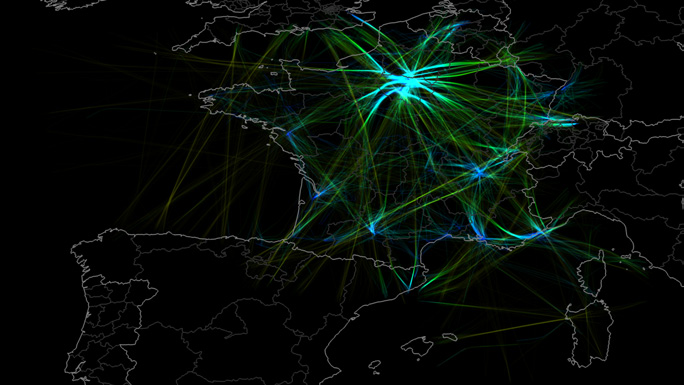
\includegraphics[width=70mm]{../figuras/air-traffic.png}
    \caption{}
  \end{subfigure}
  ~
  \begin{subfigure}[t]{0.45\textwidth}
    \centering
    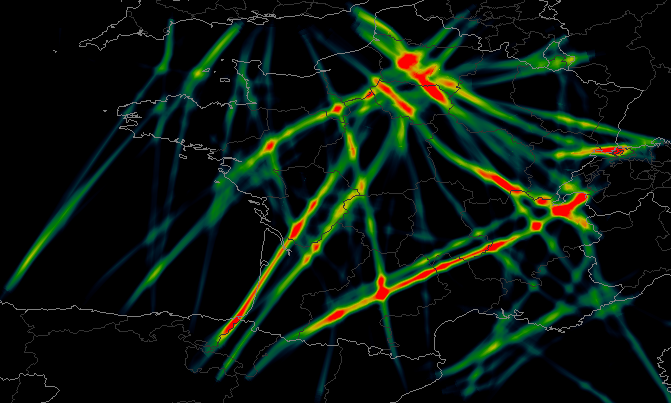
\includegraphics[width=65mm]{../figuras/klein.png}
    \caption{}
  \end{subfigure}

  \caption[Visualização do tráfego aéreo na França com
\emph{bundling}]{Visualização do tráfego aéreo na França com \emph{bundling}.
(a) Visualização da altitude. (b) Visualização de áreas congestionadas (com zoom). Fonte:
\citet{Klein2014}. \label{fig:klein}}
\end{figure}

\citet{Anita2017}~(Figura~\ref{fig:anita}) apresenta uma técnica de \emph{bundling}, resultado de uma
otimização do algoritmo FDEB, criado por \citet{Selassie2011}. Para isso,
utilizam uma etapa de clusterização aplicada previamente nos dados, e
posteriormente aplicam o \emph{bundling} em cada cluster. Eles testaram sua
abordagem em vários conjuntos de dados com informações da migração de pessoas
entre regiões dos EUA, migração de pássaros e viagens de aviões, mostrando um
ganho entre 30\% até 50\% no desempenho do algoritmo. A vantagem da sua
abordagem é que ela pode ser utilizada em conjunto com outros métodos de
\emph{bundling}. Interessante notar que sua técnica também é capaz de separar
trajetórias em direções opostas durante o processo de \emph{bundling}, mas
utilizando técnicas diferentes do que foi utilizado por \citet{adeb}.

 \begin{figure}[!htb]
  \centering
  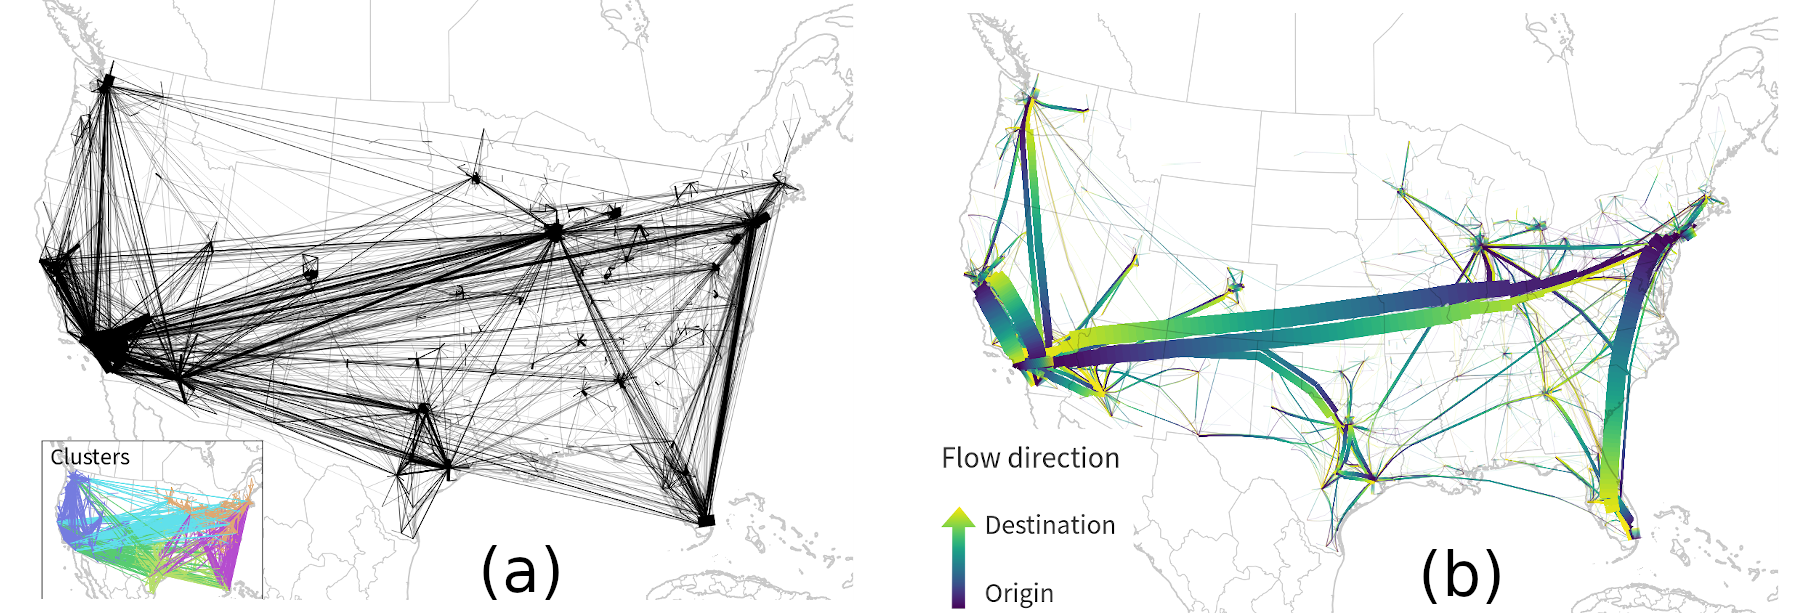
\includegraphics[width=\textwidth]{../figuras/anita.png}
  \caption[\emph{Force-Directed Edge Bundling} com clusters]{Force-Directed Edge Bundling com clusters. Fonte: \citet{Anita2017}}
   \label{fig:anita}
 \end{figure}

\citet{zeng:19} adaptaram o método KDEEB para restringir o \emph{bundling} ao
longo da rede de vias da cidade as quais os dados das trajetórias forma
coletados no que eles denominaram \emph{Road Aware Edge Bundling (RAEB)}. Sua
técnica foi demonstrada em dados contendo 166 mil viagens de táxi da cidade de
Nova Iorque. No entanto, ele requer dados detalhados das trajetórias (não apenas
OD) e também dados do leiaute das vias da cidade.

Buscamos também outros trabalhos que propõem abordagens alternativas ao
\emph{bundling}, como por exemplo, \citet{Landersberg2016}
(Figura~\ref{fig:landersberg2016}) que particionam os dados com algoritmos de
clusterização e com isso conseguem reduzir a oclusão causada pela grande
quantidade de dados. Sua técnica foi capazes de identificar diferentes padrões
de movimentação ao longo do dia e da semana. Eles demonstraram sua abordagem em
dados de geo-localização de usuários do Twitter sobre a área de Londres. Em sua
proposta, as origens e destinos são agrupadas em pontos e as linhas são
desenhadas conectando os pares de origem e destino. Para representar a direção,
eles utilizam uma escala de cores gradiente de preto para azul. Esse tipo de
abordagem agregada, no entanto, não preserva as informações de origens e
destinos das trajetórias individuais. Para complementar, eles ainda adicionam um
calendário que mostra a distribuição dos grupos e ajuda a visualizar como os
padrões de movimentação mudam ao longo das semanas (vertical) e do dia
(horizontal). Na visualização em linhas é possível ver as conexões entre
diferentes pontos da cidade e a intensidade dos fluxos. Além de técnicas de
clusterização como esta, é comum o uso de matrizes de origem-destino para
representação de grandes fluxos de movimentação, como apresentado por
\citet{Anita2017} e demonstrado na Figura~\ref{fig:anitaOD}. Esse tipo de
visualização também não permite a visualização de detalhes individuais das
trajetórias além também de perder parte da percepção de conexão
espacial entre as regiões que uma visualização baseada em linhas oferece.

 \begin{figure}[!htb]
  \centering
  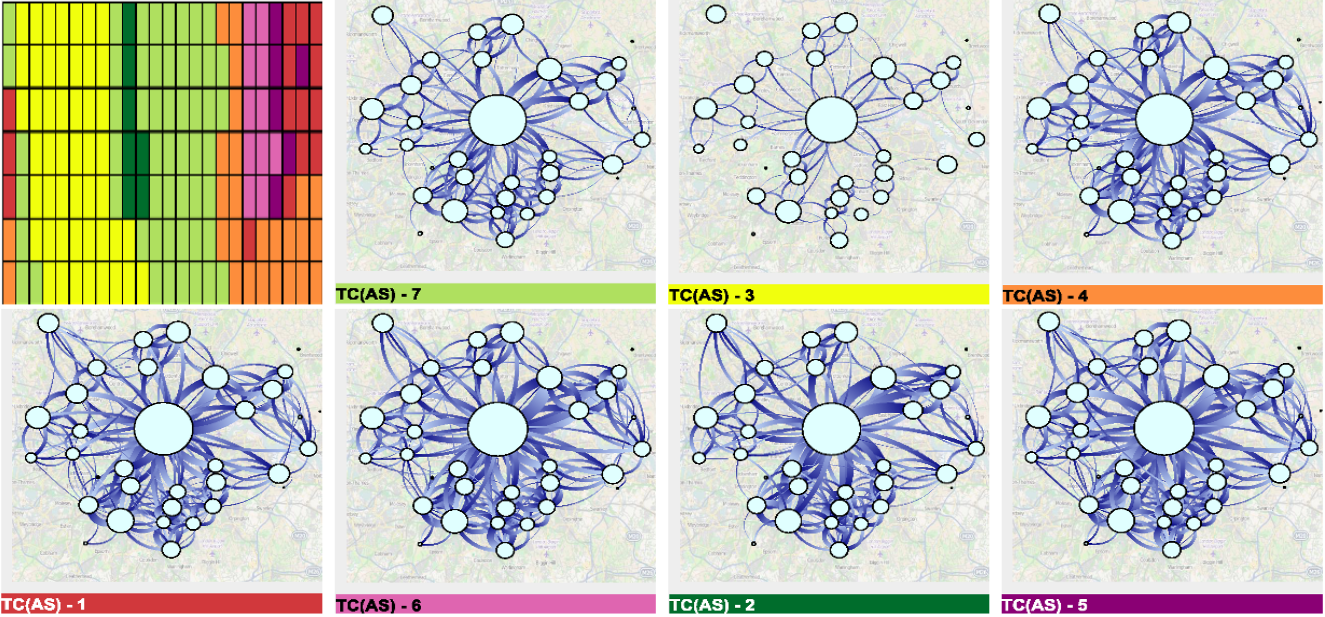
\includegraphics[width=\textwidth]{../figuras/clusters.png}
  \caption{Visualização da movimentação de usuários do Twitter em Londres. Fonte: \citet{Landersberg2016}}
   \label{fig:landersberg2016}
 \end{figure}

\begin{figure}[!htb]
  \centering
  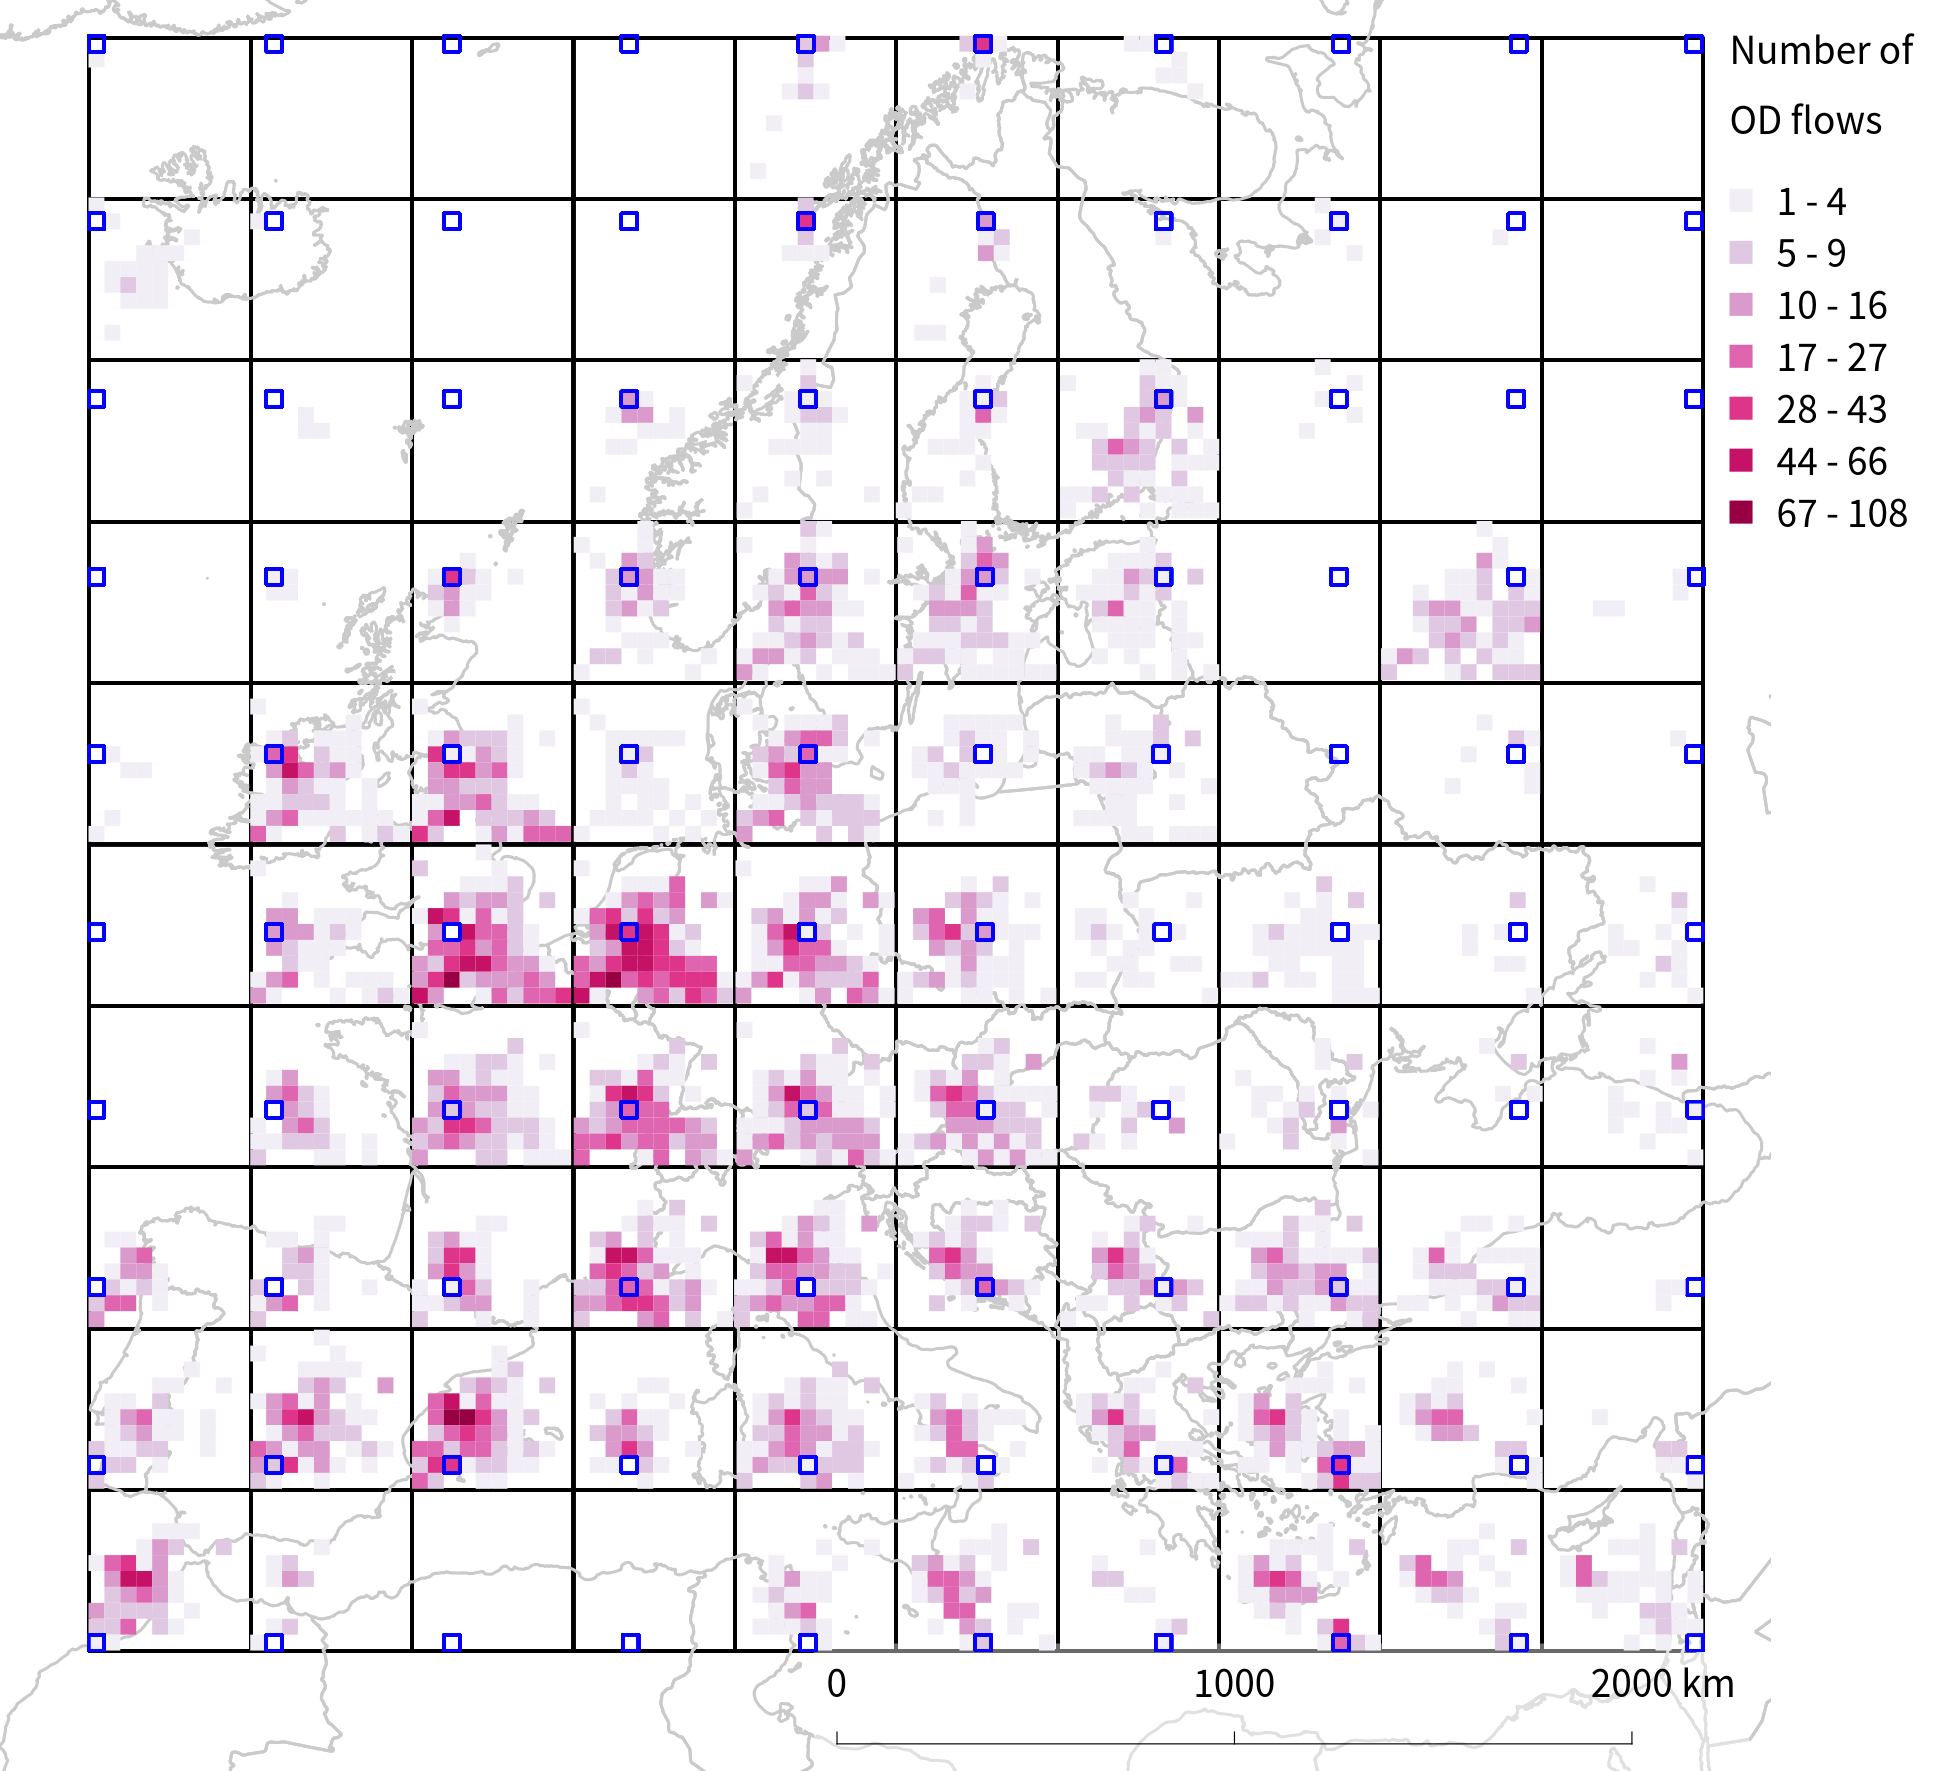
\includegraphics[width=0.8\textwidth]{../figuras/anitaOD.png}
  \caption{Matriz de Origem-Destino. As cores representam a quantidade de fluxo e os quadrados identificam a posição das regiões no mapa. Fonte: \citet{Anita2017}}
   \label{fig:anitaOD}
 \end{figure}

Não menos importante, alguns outros trabalhos que pesquisamos mostram resultados
interessantes a respeito da visualização e análise de dados de mobilidade e seus
atributos e também valem ser citados, como \citet{Ferreira2013}, que fazem uma
análise de origem e destino de 500 mil viagens de táxi feitas em um dia na
cidade de Nova Iorque. Sua visualização é baseada em pontos que destacam as
origens e destinos das viagens com cores diferentes. O resultado é similar a um
mapa de densidades que mostra a distribuição das viagens sobre a cidade.
\citet{Chu2014} também faz uma análise das trajetórias de milhares de viagens
de táxi em uma grande cidade na China para descobrir relações entre as rotas
utilizadas e relações entre ruas. Eles fazem uma transformação das latitudes e
longitudes para o nome das ruas por onde os veículos se locomovem e aplicam métodos de
clusterização e análise de texto que dão uma visão semântica das relações entre
as vias que compõe a malha rodoviária da cidade. Os resultados são mostrados em
um painel com vários tipos de visualização que utiliza mapas, gráficos e outros
recursos para exploração dos dados. \citet{Guo2011} criaram um sistema chamado
TripVista que mostra o tráfego em três perspectivas através de um painel
iterativo.  Seu sistema é focado em mostrar detalhes em nível microscópico
sobre o tráfego em cruzamentos entre ruas da cidade, como direção, quantidade
de veículos e também anomalias de motoristas que trafegam na direção contrária
da permitida. Por último \citet{Kim2018} utilizam o que eles chamam de \emph{campos
gravitacionais} para construir um mapa de fluxo de dados geoespaciais
analisando apenas as informações estatísticas da distribuições dos pontos ao
longo do tempo. Sua abordagem, no entanto implica uma série de restrições
estatísticas nos dados, como número mínimo de amostras e distribuição uniforme
dos dados ao longo do tempo.

Em nossa revisão, buscamos obter um panorama geral das lacunas que podem ser
preenchidas em relação ao uso de \emph{bundling} na visualização de fluxos de
mobilidade urbana e entender também técnicas alternativas existentes na
literatura. Entendemos que nossa abordagem contribui com um novo cenário para
utilização das técnicas de \emph{bundling} na análise de fluxos de mobilidade
urbana. Oferecemos uma análise singular da mobilidade na Região Metropolitana de
São Paulo e avançamos na investigação do \emph{CUBu} ao adaptá-lo para esse
contexto, tanto com relação aos seus parâmetros, quanto com novos recursos que
adicionamos para visualização de diferentes atributos dos dados. Além disso, a
aplicação do \emph{bundling} para visualizar um cenário de 42 milhões de
trajetórias (que em nossa metodologia reduzimos para \num{685115}) é algo que
parece ser inédito na literatura. Nesse quesito, um ponto adicional em favor do
uso do \emph{bundling} em nossa análise é que ele foi testado de maneira
relevante em grandes conjuntos de dados com centenas de milhares de dados, como
posto em \citet{Telea2018, Lhuillier2017}, o que não necessariamente é atestado
para outros métodos que citamos, segundo a nossa revisão da literatura.  No
próximo capítulo apresentamos a metodologia para o desenvolvimento de nossa
proposta.